\documentclass[graybox,natbib,nospthms]{svmono}
\usepackage{lmodern}
\usepackage{amssymb,amsmath}
\usepackage{ifxetex,ifluatex}
\usepackage{fixltx2e} % provides \textsubscript
\ifnum 0\ifxetex 1\fi\ifluatex 1\fi=0 % if pdftex
  \usepackage[T1]{fontenc}
  \usepackage[utf8]{inputenc}
\else % if luatex or xelatex
  \ifxetex
    \usepackage{mathspec}
  \else
    \usepackage{fontspec}
  \fi
  \defaultfontfeatures{Ligatures=TeX,Scale=MatchLowercase}
    \setmonofont[Mapping=tex-ansi,Scale=0.7]{Source Code Pro}
\fi
% use upquote if available, for straight quotes in verbatim environments
\IfFileExists{upquote.sty}{\usepackage{upquote}}{}
% use microtype if available
\IfFileExists{microtype.sty}{%
\usepackage{microtype}
\UseMicrotypeSet[protrusion]{basicmath} % disable protrusion for tt fonts
}{}
\usepackage[paperwidth=18.90cm, paperheight=24.58cm, top=2.1cm, bottom=2.1cm,
inner=2cm, outer=2cm,]{geometry}
\usepackage{hyperref}
\PassOptionsToPackage{usenames,dvipsnames}{color} % color is loaded by hyperref
\hypersetup{unicode=true,
            pdftitle={Predictive Soil Mapping with R},
            pdfauthor={Tomislav Hengl and Robert A. MacMillan},
            colorlinks=true,
            linkcolor=Maroon,
            citecolor=Blue,
            urlcolor=Blue,
            breaklinks=true}
\urlstyle{same}  % don't use monospace font for urls
\usepackage{color}
\usepackage{fancyvrb}
\newcommand{\VerbBar}{|}
\newcommand{\VERB}{\Verb[commandchars=\\\{\}]}
\DefineVerbatimEnvironment{Highlighting}{Verbatim}{commandchars=\\\{\}}
% Add ',fontsize=\small' for more characters per line
\usepackage{framed}
\definecolor{shadecolor}{RGB}{248,248,248}
\newenvironment{Shaded}{\begin{snugshade}}{\end{snugshade}}
\newcommand{\KeywordTok}[1]{\textcolor[rgb]{0.13,0.29,0.53}{\textbf{#1}}}
\newcommand{\DataTypeTok}[1]{\textcolor[rgb]{0.13,0.29,0.53}{#1}}
\newcommand{\DecValTok}[1]{\textcolor[rgb]{0.00,0.00,0.81}{#1}}
\newcommand{\BaseNTok}[1]{\textcolor[rgb]{0.00,0.00,0.81}{#1}}
\newcommand{\FloatTok}[1]{\textcolor[rgb]{0.00,0.00,0.81}{#1}}
\newcommand{\ConstantTok}[1]{\textcolor[rgb]{0.00,0.00,0.00}{#1}}
\newcommand{\CharTok}[1]{\textcolor[rgb]{0.31,0.60,0.02}{#1}}
\newcommand{\SpecialCharTok}[1]{\textcolor[rgb]{0.00,0.00,0.00}{#1}}
\newcommand{\StringTok}[1]{\textcolor[rgb]{0.31,0.60,0.02}{#1}}
\newcommand{\VerbatimStringTok}[1]{\textcolor[rgb]{0.31,0.60,0.02}{#1}}
\newcommand{\SpecialStringTok}[1]{\textcolor[rgb]{0.31,0.60,0.02}{#1}}
\newcommand{\ImportTok}[1]{#1}
\newcommand{\CommentTok}[1]{\textcolor[rgb]{0.56,0.35,0.01}{\textit{#1}}}
\newcommand{\DocumentationTok}[1]{\textcolor[rgb]{0.56,0.35,0.01}{\textbf{\textit{#1}}}}
\newcommand{\AnnotationTok}[1]{\textcolor[rgb]{0.56,0.35,0.01}{\textbf{\textit{#1}}}}
\newcommand{\CommentVarTok}[1]{\textcolor[rgb]{0.56,0.35,0.01}{\textbf{\textit{#1}}}}
\newcommand{\OtherTok}[1]{\textcolor[rgb]{0.56,0.35,0.01}{#1}}
\newcommand{\FunctionTok}[1]{\textcolor[rgb]{0.00,0.00,0.00}{#1}}
\newcommand{\VariableTok}[1]{\textcolor[rgb]{0.00,0.00,0.00}{#1}}
\newcommand{\ControlFlowTok}[1]{\textcolor[rgb]{0.13,0.29,0.53}{\textbf{#1}}}
\newcommand{\OperatorTok}[1]{\textcolor[rgb]{0.81,0.36,0.00}{\textbf{#1}}}
\newcommand{\BuiltInTok}[1]{#1}
\newcommand{\ExtensionTok}[1]{#1}
\newcommand{\PreprocessorTok}[1]{\textcolor[rgb]{0.56,0.35,0.01}{\textit{#1}}}
\newcommand{\AttributeTok}[1]{\textcolor[rgb]{0.77,0.63,0.00}{#1}}
\newcommand{\RegionMarkerTok}[1]{#1}
\newcommand{\InformationTok}[1]{\textcolor[rgb]{0.56,0.35,0.01}{\textbf{\textit{#1}}}}
\newcommand{\WarningTok}[1]{\textcolor[rgb]{0.56,0.35,0.01}{\textbf{\textit{#1}}}}
\newcommand{\AlertTok}[1]{\textcolor[rgb]{0.94,0.16,0.16}{#1}}
\newcommand{\ErrorTok}[1]{\textcolor[rgb]{0.64,0.00,0.00}{\textbf{#1}}}
\newcommand{\NormalTok}[1]{#1}
\usepackage{graphicx,grffile}
\makeatletter
\def\maxwidth{\ifdim\Gin@nat@width>\linewidth\linewidth\else\Gin@nat@width\fi}
\def\maxheight{\ifdim\Gin@nat@height>\textheight\textheight\else\Gin@nat@height\fi}
\makeatother
% Scale images if necessary, so that they will not overflow the page
% margins by default, and it is still possible to overwrite the defaults
% using explicit options in \includegraphics[width, height, ...]{}
\setkeys{Gin}{width=\maxwidth,height=\maxheight,keepaspectratio}
\IfFileExists{parskip.sty}{%
\usepackage{parskip}
}{% else
\setlength{\parindent}{0pt}
\setlength{\parskip}{6pt plus 2pt minus 1pt}
}
\setlength{\emergencystretch}{3em}  % prevent overfull lines
\providecommand{\tightlist}{%
  \setlength{\itemsep}{0pt}\setlength{\parskip}{0pt}}
\setcounter{secnumdepth}{0}
% Redefines (sub)paragraphs to behave more like sections
\ifx\paragraph\undefined\else
\let\oldparagraph\paragraph
\renewcommand{\paragraph}[1]{\oldparagraph{#1}\mbox{}}
\fi
\ifx\subparagraph\undefined\else
\let\oldsubparagraph\subparagraph
\renewcommand{\subparagraph}[1]{\oldsubparagraph{#1}\mbox{}}
\fi

%%% Use protect on footnotes to avoid problems with footnotes in titles
\let\rmarkdownfootnote\footnote%
\def\footnote{\protect\rmarkdownfootnote}

%%% Change title format to be more compact
\usepackage{titling}

% Create subtitle command for use in maketitle
\newcommand{\subtitle}[1]{
  \posttitle{
    \begin{center}\large#1\end{center}
    }
}

\setlength{\droptitle}{-2em}

  \title{Predictive Soil Mapping with R}
    \pretitle{\vspace{\droptitle}\centering\huge}
  \posttitle{\par}
    \author{Tomislav Hengl and Robert A. MacMillan}
    \preauthor{\centering\large\emph}
  \postauthor{\par}
      \predate{\centering\large\emph}
  \postdate{\par}
    \date{2019-02-07}


\begin{document}
\maketitle

\section*{Predictive Soil Mapping for advanced R
users}\label{predictive-soil-mapping-for-advanced-r-users}
\addcontentsline{toc}{section}{Predictive Soil Mapping for advanced R
users}

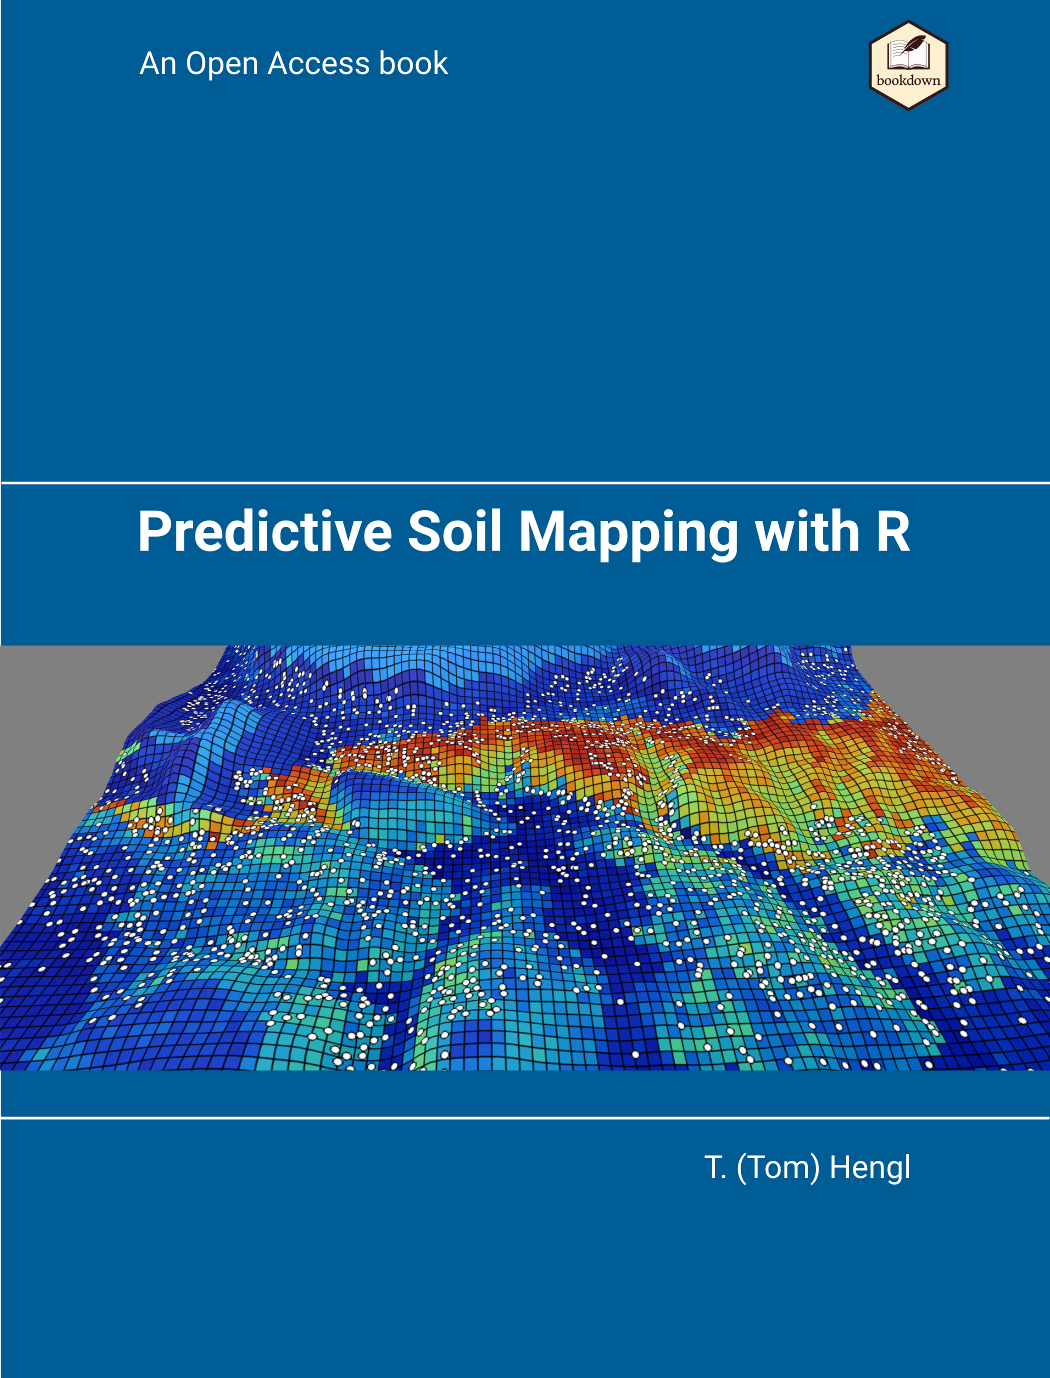
\includegraphics[width=0.33\linewidth]{figures/f0_web}

This is the online version of the Open Access book:
\href{https://envirometrix.github.io/PredictiveSoilMapping/}{\textbf{Predictive
Soil Mapping with R}}. Pull requests and general comments are welcome.
These materials are based on technical tutorials initially developed by
the \href{http://isric.org/}{ISRIC's} Global Soil Information Facilities
(GSIF) development team over the period 2014--2017.

\textbf{This book is continuously updated}. For news and updates please
refer to the
\href{https://github.com/envirometrix/PredictiveSoilMapping/issues}{github
issues}.

Hard copies of this book can be ordered from www.lulu.com.

\textbf{Cite this as}:

\begin{itemize}
\tightlist
\item
  Hengl, T., MacMillan, R.A., (2019). \textbf{Predictive Soil Mapping
  with R}. OpenGeoHub foundation, Wageningen, the Netherlands, 376
  pages, www.soilmapper.org, ISBN: 978-0-359-30635-0.
\end{itemize}

\subsection*{Editors}\label{editors}
\addcontentsline{toc}{subsection}{Editors}

\href{https://opengeohub.org/people/tom-hengl}{\textbf{Tom Hengl}} is a
Senior Researcher and Vice Chair of the OpenGeoHub Foundation /
technical director at Envirometrix Ltd. Tom has more than 20 years of
experience as an environmental modeler, data scientist and spatial
analyst. He is a passionate advocate for, and supporter of, open data,
reproducible science and career development for young scientists. He
designed and implemented the global
\href{http://journals.plos.org/plosone/article?id=10.1371/journal.pone.0169748}{SoilGrids}
data set, partially in response to other well known open data projects
such as OpenStreetMap, GBIF, GlobalForestWatch and global climate
mapping projects. He has taught predictive soil mapping at Wageningen
University / ISRIC within the ``Hands-on-GSIF'' block courses. Video
tutorials on predictive soil mapping with R can also be found at
\url{http://youtube.com/c/ISRICorg} and
\url{https://www.youtube.com/c/OpenGeoHubFoundation}. Tom currently
leads the production of a web mapping system called ``LandGIS''
(\url{https://landgis.opengeohub.org}) which is envisaged as \emph{``an
OpenStreetMap-type system''} for land-related environmental data. The
system hosts global, fine spatial resolution data (250 m to 1 km)
including various soil classes and soil properties, which is intended
for eventual integration and use at operational or farm-scales.

\href{https://opengeohub.org/people/bob-macmillan}{\textbf{Bob
MacMillan}} is a retired environmental consultant with over 40 years of
experience in creating, packaging, delivering and using environmental
information on soils, ecosystems, landforms and hydrology. Bob spent 19
years working in public sector research with the Alberta Research
Council and Agriculture and Agri-Food Canada and a second 20 years as a
private sector consultant offering services in predictive soil and
ecological mapping. Since retiring, Bob has remained an active
supporter, promoter, advocate, mentor and technical contributor to
several continental to global scale efforts to advance the science and
technology of mapping soils and other ecosystem components. As Science
Coordinator for the GlobalSoilMap project, Bob helped to articulate the
vision for the project and led initial activities aimed at achieving
this, including authoring technical specifications, promoting the
project, recruiting participants/cooperators, and liaising with
representatives of national and international soil agencies. Bob
continues to contribute on a voluntary basis to OpenGeoHub and the
Africa Soil Information Servicce (AfSIS) (\url{http://africasoils.net}).
Throughout his career, Bob has shared his expertise and his enthusiasm
freely with dozens of younger scientists interested in learning about,
and becoming, practitioners of digital soil mapping. Bob continues to
support the next generation of digital soil mappers through his
involvement with OpenGeoHub.

\section*{Preface}\label{preface}
\addcontentsline{toc}{section}{Preface}

Predictive Soil Mapping (PSM) is based on applying statistical and/or
machine learning techniques to fit models for the purpose of producing
spatial and/or spatiotemporal predictions of soil variables, i.e.~maps
of soil properties and classes at different resolutions. It is a
multidisciplinary field combining statistics, data science, soil
science, physical geography, remote sensing, geoinformation science and
a number of other sciences (Scull et al.
\protect\hyperlink{ref-Scul01}{2003}; McBratney, Mendonça Santos, and
Minasny \protect\hyperlink{ref-MCBRATNEY20033}{2003}; Henderson et al.
\protect\hyperlink{ref-Henderson2004Geoderma}{2004}; Boettinger et al.
\protect\hyperlink{ref-Boettinger2010Springer}{2010}; A. Zhu et al.
\protect\hyperlink{ref-Zhu2015PSM}{2015}). \emph{Predictive Soil Mapping
with R} is about understanding the main concepts behind soil mapping,
mastering R packages that can be used to produce high quality soil maps,
and about optimizing all processes involved so that production costs can
also be reduced.

The main differences between predictive vs traditional expert-based soil
mapping are that: (a) the production of maps is based on using
state-of-the-art statistical methods to ensure objectivity of maps
(including objective uncertainty assessment vs expert judgment), and (b)
PSM is driven by automation of the processes so that overall soil data
production costs can be reduced and updates of maps implemented without
requirements for large investments. R, in that sense, is a logical
platform to develop PSM workflows and applications, especially thanks to
the vibrant and productive R spatial interest group activities and also
thanks to the increasingly professional soil data packages such as, for
example: soiltexture, aqp, soilprofile, soilDB and similar.

The book is divided into sections covering theoretical concepts,
preparation of covariates, model selection and evaluation, prediction
and final practical tips for operational PSM. Most of the chapters
contain R code examples that try to illustrate the main processing steps
and give practical instructions to developers and applied users.

\subsection*{Connected publications}\label{connected-publications}
\addcontentsline{toc}{subsection}{Connected publications}

Most of methods described in this book are based on the following
publications:

\begin{itemize}
\item
  Hengl, T., Nussbaum, M., Wright, M. N., Heuvelink, G. B., and Gräler,
  B. (2018) \href{https://doi.org/10.7717/peerj.5518}{Random Forest as a
  generic framework for predictive modeling of spatial and
  spatio-temporal variables}. PeerJ 6:e5518.
\item
  Sanderman, J., Hengl, T., Fiske, G., (2017)
  \href{http://www.pnas.org/content/early/2017/08/15/1706103114.full}{The
  soil carbon debt of 12,000 years of human land use}. PNAS,
  \url{doi:10.1073/pnas.1706103114}
\item
  Ramcharan, A., Hengl, T., Nauman, T., Brungard, C., Waltman, S.,
  Wills, S., \& Thompson, J. (2018).
  \href{https://dl.sciencesocieties.org/publications/sssaj/abstracts/82/1/186}{Soil
  Property and Class Maps of the Conterminous United States at 100-Meter
  Spatial Resolution}. Soil Science Society of America Journal, 82(1),
  186--201.
\item
  Hengl, T., Leenaars, J. G., Shepherd, K. D., Walsh, M. G., Heuvelink,
  G. B., Mamo, T., et al. (2017)
  \href{https://link.springer.com/article/10.1007/s10705-017-9870-x}{Soil
  nutrient maps of Sub-Saharan Africa: assessment of soil nutrient
  content at 250 m spatial resolution using machine learning}. Nutrient
  Cycling in Agroecosystems, 109(1), 77--102.
\item
  Hengl T, Mendes de Jesus J, Heuvelink GBM, Ruiperez Gonzalez M,
  Kilibarda M, Blagotic A, et al. (2017)
  \href{http://dx.doi.org/10.1371/journal.pone.0169748}{SoilGrids250m:
  Global gridded soil information based on machine learning}. PLoS ONE
  12(2): e0169748. \url{doi:10.1371/journal.pone.0169748}
\item
  Shangguan, W., Hengl, T., de Jesus, J. M., Yuan, H., \& Dai, Y.
  (2017). \href{https://doi.org/10.1002/2016MS000686}{Mapping the global
  depth to bedrock for land surface modeling}. Journal of Advances in
  Modeling Earth Systems, 9(1), 65-88.
\item
  Hengl, T., Roudier, P., Beaudette, D., \& Pebesma, E. (2015)
  \href{https://www.jstatsoft.org/article/view/v063i05}{plotKML:
  scientific visualization of spatio-temporal data}. Journal of
  Statistical Software, 63(5).
\item
  Gasch, C. K., Hengl, T., Gräler, B., Meyer, H., Magney, T. S., \&
  Brown, D. J. (2015)
  \href{https://doi.org/10.1016/j.spasta.2015.04.001}{Spatio-temporal
  interpolation of soil water, temperature, and electrical conductivity
  in 3D+ T: The Cook Agronomy Farm data set}. Spatial Statistics, 14,
  70--90.
\item
  Hengl, T., Nikolic, M., \& MacMillan, R. A. (2013)
  \href{https://doi.org/10.1016/j.jag.2012.02.005}{Mapping efficiency
  and information content}. International Journal of Applied Earth
  Observation and Geoinformation, 22, 127--138.
\item
  Hengl, T., Heuvelink, G. B., \& Rossiter, D. G. (2007)
  \href{https://doi.org/10.1016/j.cageo.2007.05.001}{About
  regression-kriging: from equations to case studies}. Computers \&
  geosciences, 33(10), 1301-1315.
\item
  Hengl, T. (2006)
  \href{https://doi.org/10.1016/j.cageo.2005.11.008}{Finding the right
  pixel size}. Computers \& geosciences, 32(9), 1283--1298.
\end{itemize}

Some other relevant publications / books on the subject of Predictive
Soil Mapping and Data Science in general include:

\begin{itemize}
\item
  Malone, B.P, Minasny, B., McBratney, A.B., (2016)
  \href{https://www.springer.com/gp/book/9783319443256}{\textbf{Using R
  for Digital Soil Mapping}}. Progress in Soil Science ISBN:
  9783319443270, 262 pages.
\item
  Hengl, T., \& MacMillan, R. A. (2009).
  \href{https://doi.org/10.1016/S0166-2481(08)00019-6}{\textbf{Geomorphometry---a
  key to landscape mapping and modelling}}. Developments in Soil
  Science, 33, 433--460.
\item
  California Soil Resource Lab, (2017)
  \href{https://casoilresource.lawr.ucdavis.edu/software/}{\textbf{Open
  Source Software Tools for Soil Scientists}}, UC Davis.
\item
  McBratney, A.B., Minasny, B., Stockmann, U. (Eds) (2018)
  \href{https://www.springer.com/gp/book/9783319634371}{\textbf{Pedometrics}}.
  Progress in Soil Science ISBN: 9783319634395, 720 pages.
\item
  FAO, (2018)
  \href{https://github.com/FAO-GSP/SOC-Mapping-Cookbook}{\textbf{Soil
  Organic Carbon Mapping Cookbook}}. 2nd edt. ISBN: 9789251304402
\end{itemize}

Readers are also encouraged to obtain and study the following R books
before following some of the more complex exercises in this book:

\begin{itemize}
\item
  Bivand, R., Pebesma, E., Rubio, V., (2013)
  \href{http://www.asdar-book.org}{\textbf{Applied Spatial Data Analysis
  with R}}. Use R Series, Springer, Heidelberg, 2nd Ed. 400 pages.
\item
  Irizarry, R.A., (2018)
  \href{https://rafalab.github.io/dsbook/}{\textbf{Introduction to Data
  Science: Data Analysis and Prediction Algorithms with R}}. HarvardX
  Data Science Series.
\item
  Kabacoff, R.I., (2011)
  \href{http://www.manning.com/kabacoff/}{\textbf{R in Action: Data
  Analysis and Graphics with R}}. Manning publications, ISBN:
  9781935182399, 472 pages.
\item
  Kuhn, M., Johnson, K. (2013)
  \href{http://appliedpredictivemodeling.com}{\textbf{Applied Predictive
  Modeling}}. Springer Science, ISBN: 9781461468493, 600 pages.
\item
  Lovelace, R., Nowosad, J., Muenchow, J., (2018)
  \href{https://geocompr.robinlovelace.net}{\textbf{Geocomputation with
  R}}. R Series, CRC Press, ISBN: 9781138304512, 338 pages.
\item
  Reimann, C., Filzmoser, P., Garrett, R., Dutter, R., (2008)
  \href{https://onlinelibrary.wiley.com/doi/book/10.1002/9780470987605}{\textbf{Statistical
  Data Analysis Explained Applied Environmental Statistics with R}}.
  Wiley, Chichester, 337 pages.
\item
  Wilke, C.O., (2019)
  \href{https://serialmentor.com/dataviz/}{\textbf{Fundamentals of Data
  Visualization}}. O'Reilly, in press.
\item
  Wikle, C.K., Zammit-Mangion, A., and Cressie, N. (2019).
  \href{https://spacetimewithr.org}{\textbf{Spatio-Temporal Statistics
  with R}}. Chapman \& Hall/CRC, Boca Raton, FL.
\end{itemize}

For the most recent developments in the R-spatial community refer to
\url{https://r-spatial.github.io}, the R-sig-geo mailing list and/or
\url{https://opengeohub.org}.

\subsection*{Contributions}\label{contributions}
\addcontentsline{toc}{subsection}{Contributions}

This book is designed to be constantly updated and contributions are
always welcome (through pull requests, but also through adding new
chapters) provided that some minimum requirements are met. To contribute
a new chapter please contact the editors first. Some minimum
requirements to contribute a chapter are:

\begin{enumerate}
\def\labelenumi{\arabic{enumi}.}
\tightlist
\item
  The data needs to be available for the majority of tutorials presented
  in a chapter. It is best if this is via some R package or web-source.
\item
  A chapter should ideally focus on implementing some computing in R (it
  should be written as an R tutorial).
\item
  All examples should be computationally efficient requiring not more
  than 30 secs of computing time per process on a single core system.
\item
  The theoretical basis for methods and interpretation of results should
  be based on peer-review publications. This book is not intended to
  report on primary research / experimental results, but only to
  supplement existing research publications.
\item
  A chapter should consist of at least 1500 words and at most 3500
  words.
\item
  The topic of the chapter must be closely connected to the theme of
  soil mapping, soil geographical databases, methods for processing
  spatial soil data and similar.
\end{enumerate}

In principle, all submitted chapters should follow closely also the
\href{https://en.wikipedia.org/wiki/Wikipedia:Five_pillars}{five pillars
of Wikipedia}, especially: Verifiability, Reproducibility, No original
research, Neutral point of view, Good faith, No conflict of interest,
and No personal attacks.

\subsection*{Reproducibility}\label{reproducibility}
\addcontentsline{toc}{subsection}{Reproducibility}

To reproduce the book, you need a recent version of
\href{https://cran.r-project.org}{R}, and
\href{http://www.rstudio.com/products/RStudio/}{RStudio} and up-to-date
packages, which can be installed with the following command (which
requires \href{https://github.com/hadley/devtools}{\textbf{devtools}}):

\begin{Shaded}
\begin{Highlighting}[]
\NormalTok{devtools}\OperatorTok{::}\KeywordTok{install_github}\NormalTok{(}\StringTok{"Envirometrix/PSMpkg"}\NormalTok{)}
\end{Highlighting}
\end{Shaded}

To build the book locally, clone or
\href{https://github.com/envirometrix/PredictiveSoilMapping/archive/master.zip}{download}
the
\href{https://github.com/envirometrix/PredictiveSoilMapping/}{PredictiveSoilMapping
repo}, load R in root directory (e.g.~by opening
\href{https://github.com/envirometrix/PredictiveSoilMapping/blob/master/PredictiveSoilMapping.Rproj}{PredictiveSoilMapping.Rproj}
in RStudio) and run the following lines:

\begin{Shaded}
\begin{Highlighting}[]
\NormalTok{bookdown}\OperatorTok{::}\KeywordTok{render_book}\NormalTok{(}\StringTok{"index.Rmd"}\NormalTok{) }\CommentTok{# to build the book}
\KeywordTok{browseURL}\NormalTok{(}\StringTok{"docs/index.html"}\NormalTok{) }\CommentTok{# to view it}
\end{Highlighting}
\end{Shaded}

\subsection*{Acknowledgements}\label{acknowledgements}
\addcontentsline{toc}{subsection}{Acknowledgements}

The authors are grateful for numerous contributions from colleagues
around the world, especially for contributions by current and former
ISRIC --- World Soil Information colleagues and guest researchers:
Gerard Heuvelink, Johan Leenaars, Jorge Mendes de Jesus, Wei Shangguan,
David G. Rossiter, and many others. The authors are also grateful to
Dutch and European citizens for financing ISRIC and Wageningen
University, where work on this book was initially started. The authors
acknowledge support received from the
\href{http://africasoils.net}{AfSIS project}, which was funded by the
Bill and Melinda Gates Foundation (BMGF) and the Alliance for a Green
Revolution in Africa (AGRA). Many soil data processing examples in the
book are based on R code developed by Dylan Beuadette, Pierre Roudier,
Alessandro Samuel Rosa, Marcos E. Angelini, Guillermo Federico Olmedo,
Julian Moeys, Brandon Malone, and many other developers. The authors are
also grateful to comments and suggestions for improvements to the
methods presented in the book by Travis Nauman, Amanda Ramcharan, David
G. Rossiter and \href{http://julienmoeys.info}{Julian Moeys}.

LandGIS and SoilGrids are based on using numerous soil profile data sets
kindly made available by various national and international agencies:
the USA National Cooperative Soil Survey Soil Characterization database
(\url{http://ncsslabdatamart.sc.egov.usda.gov}) and profiles from the
USA National Soil Information System, Land Use/Land Cover Area Frame
Survey (LUCAS) Topsoil Survey database (Tóth, Jones, and Montanarella
\protect\hyperlink{ref-Toth2013LUCAS}{2013}), Repositório Brasileiro
Livre para Dados Abertos do Solo
(\href{https://github.com/febr-team}{FEBR}), Sistema de Información de
Suelos de Latinoamérica y el Caribe (SISLAC), Africa Soil Profiles
database (Leenaars \protect\hyperlink{ref-Leenaars2012}{2014}),
Australian National Soil Information by CSIRO Land and Water (Karssies
\protect\hyperlink{ref-Karssies2011CSIRO}{2011}; Searle
\protect\hyperlink{ref-searle2014australian}{2014}), Mexican National
soil profile database (Instituto Nacional de Estadística y Geografía
(INEGI) \protect\hyperlink{ref-INEGI2000}{2000}) provided by the Mexican
Instituto Nacional de Estadística y Geografía / CONABIO, Brazilian
national soil profile database (Cooper et al.
\protect\hyperlink{ref-cooper2005national}{2005}) provided by the
University of São Paulo, Chinese National Soil Profile database
(Shangguan et al. \protect\hyperlink{ref-shangguan2013china}{2013})
provided by the Institute of Soil Science, Chinese Academy of Sciences,
soil profile archive from the Canadian Soil Information System
(MacDonald and Valentine
\protect\hyperlink{ref-macdonald1992cansis}{1992}) and Forest Ecosystem
Carbon Database (FECD), ISRIC-WISE (Batjes
\protect\hyperlink{ref-Batjes2009SUM}{2009}), The Northern Circumpolar
Soil Carbon Database (Hugelius et al.
\protect\hyperlink{ref-essd-5-3-2013}{2013}), eSOTER profiles (Van
Engelen and Dijkshoorn \protect\hyperlink{ref-VanEngelen2012}{2012}),
SPADE (Hollis et al. \protect\hyperlink{ref-hollis2006spade}{2006}),
Unified State Register of soil resources RUSSIA (Version 1.0. Moscow ---
2014), National Database of Iran provided by the Tehran University,
points from the Dutch Soil Information System (BIS) prepared by
Wageningen Environmental Research, and others. We are also grateful to
USA's NASA, USGS and USDA agencies, European Space Agency Copernicus
projects, JAXA (Japan Aerospace Exploration Agency) for distributing
vast amounts of remote sensing data (especially MODIS, Landsat,
Copernicus land products and elevation data), and to the Open Source
software developers of the packages rgdal, sp, raster, caret, mlr,
ranger, SuperLearner, h2o and similar, and without which predictive soil
mapping would most likely not be possible.

This book has been inspired by
\href{https://geocompr.robinlovelace.net}{the Geocomputation with R
book}, an Open Access book edited by Robin Lovelace, Jakub Nowosad and
Jannes Muenchow. Many thanks to Robin Lovelace for helping with
rmarkdown and for giving some initial tips for compiling and organizing
this book. The authors are also grateful to the numerous
software/package developers, especially Edzer Pebesma, Roger Bivand,
Robert Hijmans, Markus Neteler, Tim Appelhans, and Hadley Wickham, whose
contributions have enabled a generation of researchers and applied
projects.

We are especially grateful to \href{https://nowosad.github.io/}{Jakub
Nowosad} for helping with preparing this publication for press and with
setting up all code so that it passes automatic checks.

OpenGeoHub is a not-for-profit research foundation with headquarters in
Wageningen, the Netherlands (Stichting OpenGeoHub, KvK 71844570). The
main goal of the OpenGeoHub is to promote publishing and sharing of Open
Geographical and Geoscientific Data and using and developing of Open
Source Software. We believe that the key measure of quality of research
in all sciences (and especially in geographical information sciences) is
in transparency and reproducibility of the computer code used to
generate results. Transparency and reproducibility increase trust in
information so that it is eventually also the fastest path to optimal
decision making.

Every effort has been made to trace copyright holders of the materials
used in this publication. Should we, despite all our efforts, have
overlooked contributors please contact the author and we shall correct
this unintentional omission without any delay and will acknowledge any
overlooked contributions and contributors in future updates.

\begin{center}\rule{0.5\linewidth}{\linethickness}\end{center}

\textbf{Data availability and Code license}: All data used in this book
is either available through R packages or is available via the github
repository. If not mentioned otherwise, all code presented is available
under the
\href{https://www.gnu.org/licenses/old-licenses/gpl-2.0.en.html}{GNU
General Public License v2.0}.

\textbf{Copyright}: © 2019 Authors.

This work is licensed under a Creative Commons Attribution-ShareAlike
4.0 International License. LandGIS and OpenGeoHub are registered
trademarks of the OpenGeoHub Foundation (\url{https://opengeohub.org}).

\hypertarget{refs}{}
\hypertarget{ref-Batjes2009SUM}{}
Batjes, N. H. 2009. ``Harmonized soil profile data for applications at
global and continental scales: Updates to the WISE database.''
\emph{Soil Use and Management} 25 (2): 124--27.
doi:\href{https://doi.org/10.1111/j.1475-2743.2009.00202.x}{10.1111/j.1475-2743.2009.00202.x}.

\hypertarget{ref-Boettinger2010Springer}{}
Boettinger, J. L., D. W. Howell, A. C. Moore, A. E. Hartemink, and S.
Kienast-Brown, eds. 2010. \emph{Digital Soil Mapping: Bridging Research,
Environmental Application, and Operation}. Vol. 2. Progress in Soil
Science. Springer.

\hypertarget{ref-cooper2005national}{}
Cooper, Miguel, Lúcia Maria Silveira Mendes, Wellinton Luiz Costa Silva,
and Gerd Sparovek. 2005. ``A National Soil Profile Database for Brazil
Available to International Scientists.'' \emph{Soil Science Society of
America Journal} 69 (3). Soil Science Society: 649--52.

\hypertarget{ref-Henderson2004Geoderma}{}
Henderson, B. L., E. N. Bui, C. J. Moran, and D. A. P. Simon. 2004.
``Australia-wide predictions of soil properties using decision trees.''
\emph{Geoderma} 124 (3-4): 383--98.

\hypertarget{ref-hollis2006spade}{}
Hollis, J. M., R. J. A. Jones, C. J. Marshall, A. Holden, J. R. Van de
Veen, and L. Montanarella. 2006. \emph{SPADE-2: The soil profile
analytical database for Europe, version 1.0}. Luxembourg: Office for
official publications of the European Communities.

\hypertarget{ref-essd-5-3-2013}{}
Hugelius, G., C. Tarnocai, G. Broll, J. G. Canadell, P. Kuhry, and D. K.
Swanson. 2013. ``The Northern Circumpolar Soil Carbon Database:
Spatially Distributed Datasets of Soil Coverage and Soil Carbon Storage
in the Northern Permafrost Regions.'' \emph{Earth System Science Data} 5
(1): 3--13.
doi:\href{https://doi.org/10.5194/essd-5-3-2013}{10.5194/essd-5-3-2013}.

\hypertarget{ref-INEGI2000}{}
Instituto Nacional de Estadística y Geografía (INEGI). 2000.
\emph{Conjunto de Datos de Perfiles de Suelos, Escala 1: 250 000 Serie
Ii}. (Continuo Nacional). Aguascalientes, Ags. México: INEGI.

\hypertarget{ref-Karssies2011CSIRO}{}
Karssies, Linda. 2011. \emph{CSIRO National Soil Archive and the
National Soil Database (Natsoil)}. Data Collection v1. Canberra: CSIRO.

\hypertarget{ref-Leenaars2012}{}
Leenaars, Johan G.B. 2014. \emph{Africa Soil Profiles Database, Version
1.2. a Compilation of Geo-Referenced and Standardized Legacy Soil
Profile Data for Sub Saharan Africa (with Dataset)}. Wageningen, the
Netherlands: Africa Soil Information Service (AfSIS) project; ISRIC ---
World Soil Information.

\hypertarget{ref-macdonald1992cansis}{}
MacDonald, K. B., and K. W. G. Valentine. 1992. \emph{CanSIS/Nsdb. a
General Description}. Ottawa: Centre for Land; Biological Resources
Research, Research Branch, Agriculture Canada.

\hypertarget{ref-MCBRATNEY20033}{}
McBratney, A.B, M.L Mendonça Santos, and B Minasny. 2003. ``On Digital
Soil Mapping.'' \emph{Geoderma} 117 (1): 3--52.
doi:\href{https://doi.org/10.1016/S0016-7061(03)00223-4}{10.1016/S0016-7061(03)00223-4}.

\hypertarget{ref-Scul01}{}
Scull, P., J. Franklin, O. A. Chadwick, and D. McArthur. 2003.
``Predictive Soil Mapping: A Review.'' \emph{Progress in Physical
Geography} 27 (2): 171--97.

\hypertarget{ref-searle2014australian}{}
Searle, R. 2014. ``The Australian Site Data Collation to Support the
Globalsoilmap.'' \emph{GlobalSoilMap: Basis of the Global Spatial Soil
Information System}. CRC Press, 127.

\hypertarget{ref-shangguan2013china}{}
Shangguan, Wei, Yongjiu Dai, Baoyuan Liu, Axing Zhu, Qingyun Duan,
Lizong Wu, Duoying Ji, et al. 2013. ``A China Data Set of Soil
Properties for Land Surface Modeling.'' \emph{Journal of Advances in
Modeling Earth Systems} 5 (2): 212--24.
doi:\href{https://doi.org/10.1002/jame.20026}{10.1002/jame.20026}.

\hypertarget{ref-Toth2013LUCAS}{}
Tóth, G., A. Jones, and L. Montanarella, eds. 2013. \emph{LUCAS Topsoil
Survey. Methodology, Data and Results}. JRC Technical Reports Eur 26102.
Luxembourg: Publications Office of the European Union.

\hypertarget{ref-VanEngelen2012}{}
Van Engelen, V.W.P., and J.A. Dijkshoorn, eds. 2012. \emph{Global and
National Soils and Terrain Digital Databases (SOTER), Procedures Manual,
version 2.0}. ISRIC Report 2012/04. Wageningen, the Netherlands: ISRIC -
World Soil Information.

\hypertarget{ref-Zhu2015PSM}{}
Zhu, A.X., J. Liu, F. Du, S.J. Zhang, C.Z. Qin, J. Burt, T. Behrens, and
T. Scholten. 2015. ``Predictive Soil Mapping with Limited Sample Data.''
\emph{European Journal of Soil Science} 66 (3): 535--47.
doi:\href{https://doi.org/10.1111/ejss.12244}{10.1111/ejss.12244}.


\end{document}
